\documentclass[tikz,border=12pt]{standalone}
\usepackage{tikz}
\usetikzlibrary{shapes.geometric, arrows.meta, positioning, calc}



\begin{document}

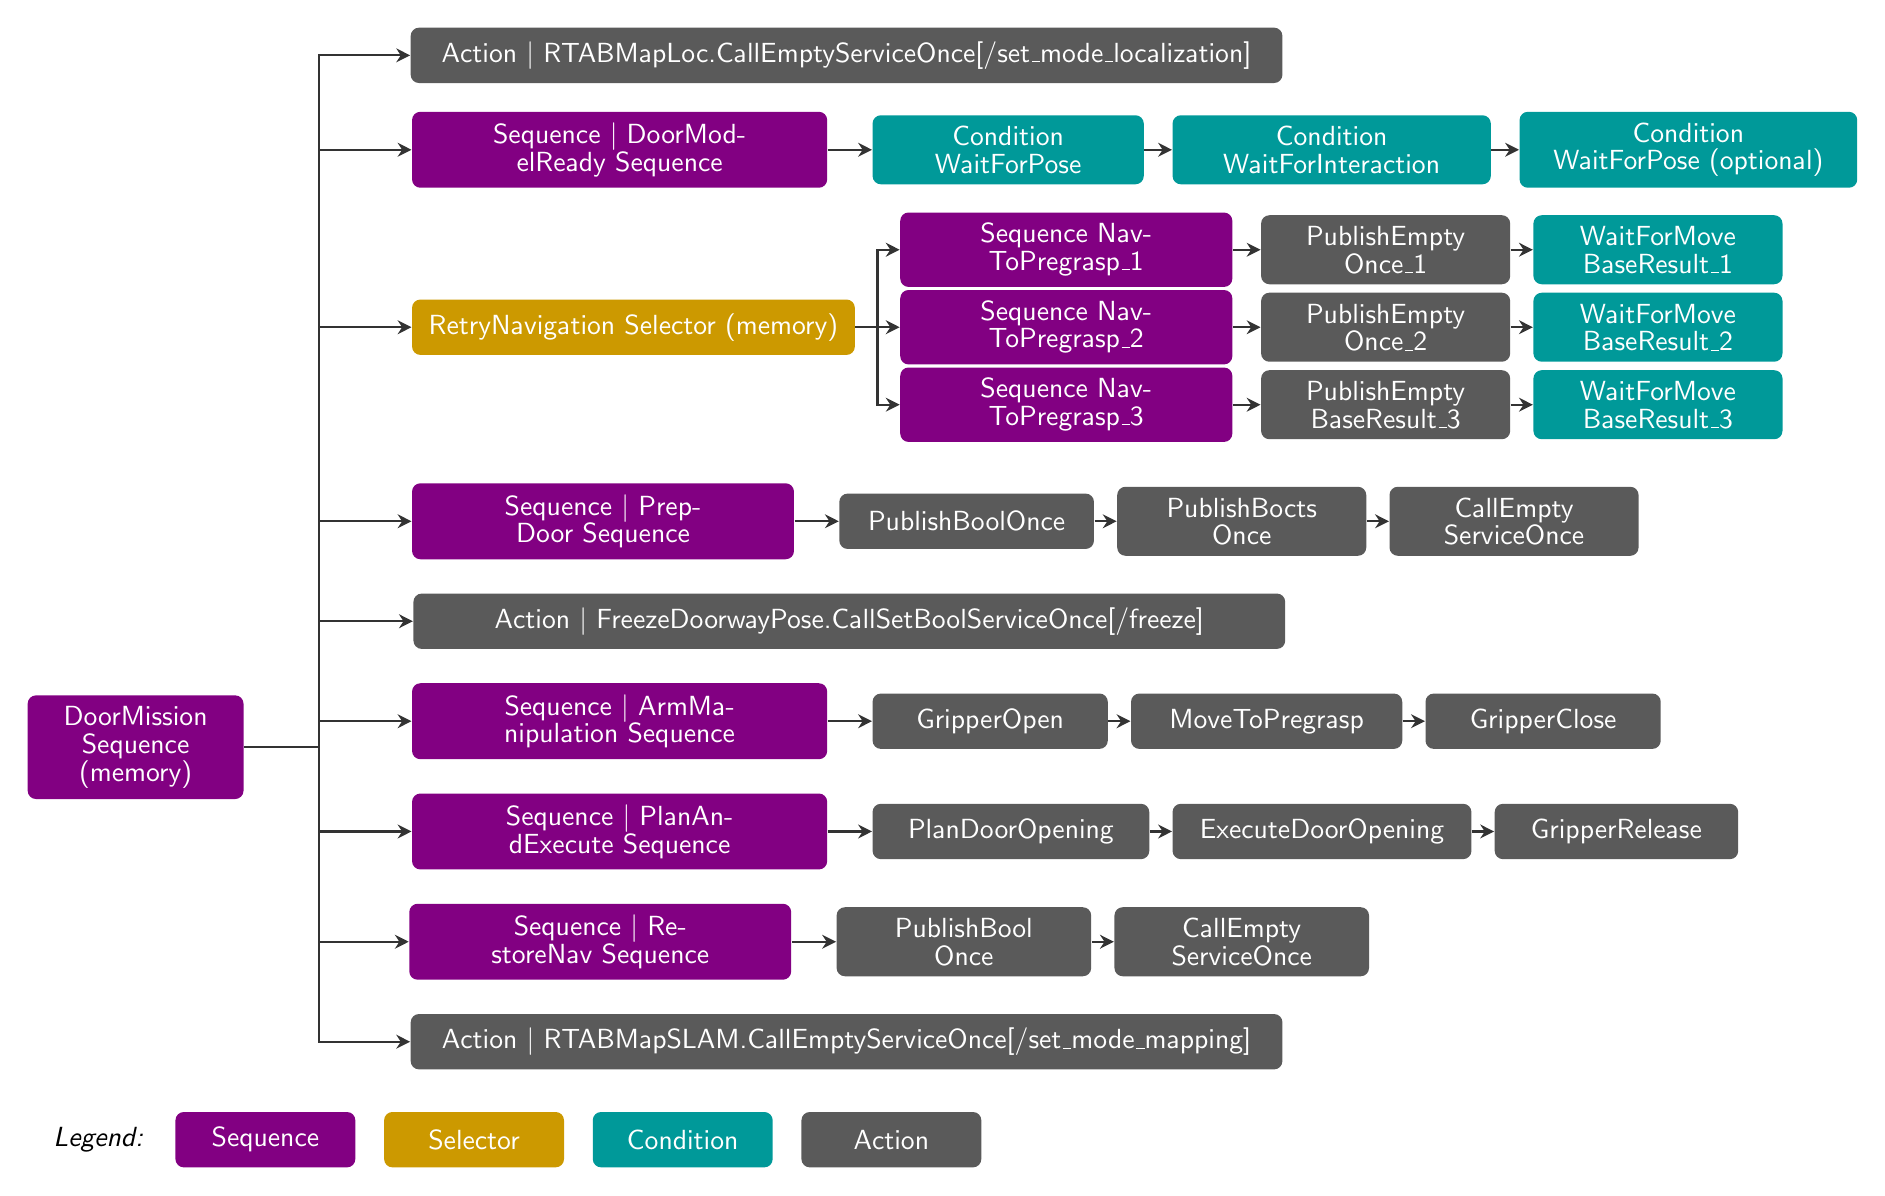
\begin{tikzpicture}[node distance = 8pt and 22pt]

% Node styles    
\tikzset{
  every node/.style={font=\fontsize{10}{10}\sffamily},
  bt/.style={
    draw=none, rounded corners=3pt, text=white,
    minimum height=20pt, inner xsep=5pt, inner ysep=4pt,
    text centered, align=center
  },
  btseq/.style={bt, fill=seqColor},
  btsel/.style={bt, fill=selColor},
  btcond/.style={bt, fill=condColor},
  btact/.style={bt, fill=actColor},
  btwact/.style={bt, fill=waitColor},
  edge/.style={-{Stealth[length=5pt,width=5pt]}, thick, draw=black!80},
}

% Colour palette
\definecolor{seqColor} {RGB}{130,  0,130}
\definecolor{selColor} {RGB}{204,153,  0}
\definecolor{condColor}{RGB}{  0,153,153}
\definecolor{actColor} {RGB}{ 90, 90, 90}
\definecolor{waitColor}{RGB}{  0,153,153}

%% ROOT
\node[btseq, text width=68pt] (root) {DoorMission\\Sequence\\(memory)};

%% Column-1

\node[btact, text width=305pt, right=60pt of root, yshift=250pt] (rtabmaploc)
  {Action \textbar\ RTABMapLoc.CallEmptyServiceOnce[/set\_mode\_localization]};

\node[btseq, text width=140pt,
      below=10pt of rtabmaploc, xshift=-82pt] (dmrseq)
  {Sequence \textbar\ DoorModelReady Sequence};

\node[btsel, text width=150pt, below=40pt of dmrseq, xshift=5pt] (retry)
  {RetryNavigation Selector (memory)};

\node[btseq, text width=128pt, below=46pt of retry, xshift=-11pt] (prepdoor)
  {Sequence \textbar\ PrepDoor Sequence};

\node[btact, text width=305pt,below=12pt of prepdoor, xshift=89pt] (freeze)
  {Action \textbar\ FreezeDoorwayPose.CallSetBoolServiceOnce[/freeze]};

\node[btseq, text width=140pt, below=12pt of freeze, xshift=-83pt] (armmanip)
  {Sequence \textbar\ ArmManipulation Sequence};

\node[btseq, text width=140pt,below=12pt of armmanip] (planexec)
  {Sequence \textbar\ PlanAndExecute Sequence};

\node[btseq, text width=128pt,
      below=12pt of planexec, xshift=-7pt] (restorenav)
  {Sequence \textbar\ RestoreNav Sequence};

\node[btact, text width=305pt,
      below=12pt of restorenav, xshift=89pt] (rtabmapslam)
  {Action \textbar\ RTABMapSLAM.CallEmptyServiceOnce[/set\_mode\_mapping]};

%% DoorModelReady children
\node[btcond, text width=88pt, right=16pt of dmrseq](wfpose1){Condition\\WaitForPose};
\node[btcond, text width=105pt, right=10pt of wfpose1](wfinteract){Condition\\WaitForInteraction};
\node[btcond, text width=112pt, right=10pt of wfinteract](wfposeopt){Condition\\WaitForPose (optional)};

%% RetryNavigation children
\node[btseq, text width=110pt, right=16pt of retry, yshift=28pt](nav1){Sequence NavToPregrasp\_1};
\node[btseq, text width=110pt, right=16pt of retry](nav2){Sequence NavToPregrasp\_2};
\node[btseq, text width=110pt, right=16pt of retry, yshift=-28pt](nav3){Sequence NavToPregrasp\_3};

\node[btact, text width=80pt, right=10pt of nav1](pub1){PublishEmpty\\Once\_1};
\node[btwact, text width=80pt, right=8pt of pub1](wfm1){WaitForMove\\BaseResult\_1};
\node[btact, text width=80pt, right=10pt of nav2](pub2){PublishEmpty\\Once\_2};
\node[btwact, text width=80pt, right=8pt of pub2](wfm2){WaitForMove\\BaseResult\_2};
\node[btact, text width=80pt, right=10pt of nav3](pub3){PublishEmpty\\BaseResult\_3};
\node[btwact, text width=80pt, right=8pt of pub3](wfm3){WaitForMove\\BaseResult\_3};

%% PrepDoor children
\node[btact, text width=82pt, right=16pt of prepdoor] (pubbool1){PublishBoolOnce};
\node[btact, text width=80pt, right=8pt of pubbool1] (pubbocts){PublishBocts\\Once};
\node[btact, text width=80pt, right=8pt of pubbocts] (callempty1){CallEmpty\\ServiceOnce};

%% ArmManipulation children
\node[btact, text width=75pt, right=16pt of armmanip](gripopen){GripperOpen};
\node[btact, text width=88pt, right=8pt of gripopen](movepregrasp){MoveToPregrasp};
\node[btact, text width=75pt, right=8pt of movepregrasp](gripclose){GripperClose};

%% PlanAndExecute children
\node[btact, text width=90pt, right=16pt of planexec](plandoor){PlanDoorOpening};
\node[btact, text width=98pt, right=8pt of plandoor](execdoor){ExecuteDoorOpening};
\node[btact, text width=78pt, right=8pt of execdoor](griprel){GripperRelease};

%% RestoreNav children
\node[btact, text width=82pt, right=16pt of restorenav](pubbool2){PublishBool\\Once};
\node[btact, text width=82pt, right=8pt of pubbool2](callempty2){CallEmpty\\ServiceOnce};

%%  EDGES

% Root to all level-1 children: short trunk, then branch vertically, then connect
\foreach \child in {rtabmaploc, dmrseq, retry, prepdoor,
                    freeze, armmanip, planexec, restorenav, rtabmapslam}{
  \draw[edge] (root.east) -- ++(27pt,0) |- (\child.west);
}

% DoorModelReady chain
\draw[edge] (dmrseq.east) -- (wfpose1.west);
\draw[edge] (wfpose1.east) -- (wfinteract.west);
\draw[edge] (wfinteract.east) -- (wfposeopt.west);

% RetryNavigation to nav sequences
\foreach \child in {nav1, nav2, nav3}{
  \draw[edge] (retry.east) -- ++(8pt,0) |- (\child.west);
}

% Nav leaf chains
\draw[edge] (nav1.east) -- (pub1.west);  \draw[edge] (pub1.east) -- (wfm1.west);
\draw[edge] (nav2.east) -- (pub2.west);  \draw[edge] (pub2.east) -- (wfm2.west);
\draw[edge] (nav3.east) -- (pub3.west);  \draw[edge] (pub3.east) -- (wfm3.west);

% PrepDoor chain
\draw[edge] (prepdoor.east) -- (pubbool1.west);
\draw[edge] (pubbool1.east) -- (pubbocts.west);
\draw[edge] (pubbocts.east) -- (callempty1.west);

% ArmManipulation chain
\draw[edge] (armmanip.east) -- (gripopen.west);
\draw[edge] (gripopen.east) -- (movepregrasp.west);
\draw[edge] (movepregrasp.east) -- (gripclose.west);

% PlanAndExecute chain
\draw[edge] (planexec.east) -- (plandoor.west);
\draw[edge] (plandoor.east) -- (execdoor.west);
\draw[edge] (execdoor.east) -- (griprel.west);

% RestoreNav chain
\draw[edge] (restorenav.east) -- (pubbool2.west);
\draw[edge] (pubbool2.east) -- (callempty2.west);


%%  LEGEND
\node[btseq, text width=55pt, below=15pt of rtabmapslam, xshift=-210pt](leg_seq){Sequence};
\node[btsel, text width=55pt, right=10pt of leg_seq](leg_sel){Selector};
\node[btcond, text width=55pt, right=10pt of leg_sel](leg_cond){Condition};
\node[btact, text width=55pt, right=10pt of leg_cond](leg_act){Action};
\node[left=8pt of leg_seq, font=\fontsize{10}{10}\sffamily\itshape, text=black]{Legend:};

\end{tikzpicture}
\end{document}